
(a) Khi chưa đảo mạch, mạch gồm: $R_S$ nt $R_1$ nt ($R_2$//$(R_3$ nt $R_L))$.

Điện trở của nhánh ra là:
\begin{equation}
    R_{3L}=R_3+R_L.
\end{equation}

Để nguồn phát hoạt động ổn định, điện trở tương đương toàn mạch $R_{\text{td}}$ phải bằng $R_S$:
\begin{equation}
    R_S=R_{\text{tđ}}=R_1+\frac{R_2 R_{3L}}{R_2+R_{3L}}
\end{equation}

Gọi $I_{in}$ là dòng điện tổng. Hiệu điện thế đầu vào $(U_{\text{in}})$:

\begin{equation}
      U_{\mathrm{in}}=\left(R_1+\frac{R_2R_{3L}}{R_2+R_{3L}}\right)I_{\mathrm{in}}.
\end{equation}

Áp dụng quy tắc chia dòng và định luật Ohm cho nhánh chứa $R_L$, hiệu điện thế đầu ra trên tải $(U_{\text{out}})$ là:

\begin{equation}
      U_{\mathrm{out}}=\frac{R_2}{R_2+R_{3L}}\,R_L\,I_{\mathrm{in}}.
\end{equation}

Dựa vào tỉ số giữa hiệu điện thể đầu ra và đầu vào, ta tính được độ suy hao của mạch:

\begin{equation}
      \frac{U_{\mathrm{out}}}{U_{\mathrm{in}}}=\frac{R_2R_L}{R_1(R_{3L}+R_2)+R_{3L}R_2}.
\end{equation}

Khi ta đổi mạch (1) và mạch (3), dòng điện sẽ đi vào từ phía $R_3$. \\ Lúc này, mạch gồm: ($R_S$ nt $R_3$) nt ($R_2$//($(R_1$ nt $R_L)$)).

Điện trở nhánh ra mới là:

\begin{equation}
    R_{\mathrm{1L}}=R_1+R_{L}.
\end{equation}

Dựa vào tỉ số giữa hiệu điện thể đầu ra và đầu vào, tương tự, ta tính được độ suy hao mới của mạch:

\begin{equation}
      \frac{U'_{\mathrm{out}}}{U'_{\mathrm{in}}}=\frac{R_2R_L}{R_3(R_{1L}+R_2)+R_{1L}R_2}.
\end{equation}

Điện trở tương đương toàn mạch sau khi đảo mạch $(R'_{\text{tđ}})$: 

\begin{equation}
      R_S=R'_{\text{tđ}}=R_3+\frac{R_2R_{1L}}{R_2+R_{1L}}.
\end{equation}

Để đảm bảo tính phối hợp trở kháng khi đảo, điện trở tương đương của mạch phải không đổi: 

\begin{equation}
    R_\text{tđ}=R'_\text{tđ}
\end{equation}

Biến đổi ta được: 
\begin{equation}
R_1+\frac{R_2(R_3+R_L)}{R_2+(R_3+R_L)}=R_3+\frac{R_2(R_1+R_L)}{R_2+(R_1+R_L)}.
\end{equation}

Ta thu được điều kiện:

\begin{equation}
    \begin{aligned}
    R_1-R_3&=0 \\    \Rightarrow R_1&=R_3
    \end{aligned}
\end{equation}

Khi $R_1=R_3=R$, thay vào hai biểu thức tỉ số suy hao đã lập ở trên:

\begin{equation}
    \frac{U_{\mathrm{out}}}{U_{\mathrm{in}}}=\frac{R_2R_L}{R(R+R_L+R_2)+R_2(R+R_L)}.
\end{equation}

\begin{equation}
    \frac{U'_{\mathrm{out}}}{U'_{\mathrm{in}}}=\frac{R_2R_L}{R(R+R_L+R_2)+R_2(R+R_L)}.
\end{equation}

Suy ra:

\begin{equation}
    \frac{U_{\mathrm{out}}}{U_{\mathrm{in}}}=\frac{U'_{\mathrm{out}}}{U'_{\mathrm{in}}}.
\end{equation}

Nếu giữ nguyên mức hiệu điện thế nguồn đầu vào $(U_{\mathrm{in}}=U'_{\mathrm{in}})$, thì hiển nhiên:

\begin{equation}
    U_{\mathrm{out}}=U'_{\mathrm{out}}.
\end{equation}

(b) Biến đổi phương trình trở kháng ($R_2$ theo $R, R_L$):

\begin{equation}
\label{eq:b1}
\begin{aligned}
    R_L
    &= R + \frac{R_2(R+R_L)}{R_2+(R+R_L)}
    \Rightarrow R_2
    &= \frac{R_L^2-R^2}{2R}
\end{aligned}
\end{equation}


Thiết lập hệ số suy hao hiệu điện thế $K=\left(\dfrac{U_{\mathrm{in}}}{U_{\mathrm{out}}}\right)$:

\begin{equation}
\begin{aligned}
K
&= \frac{U_{in}}{U_{out}} 
&= \frac{R_2+R+R_L}{R_2} 
&= 1 + \frac{R+R_L}{R_2}
\end{aligned}
\end{equation}

Thế phương trình \eqref{eq:b1} vào:

\begin{equation}
\begin{aligned}
K
&= 1 + \frac{2R(R+R_L)}{R_L^2-R^2} 
&= 1 + \frac{2R}{R_L-R} 
&= \frac{R_L+R}{R_L-R}
\end{aligned}
\end{equation}

Qua các phép biến đổi, ta tính được R theo K và $R_L$

\begin{equation}
\begin{aligned}
R
&= \frac{K-1}{K+1} R_L
\end{aligned}
\end{equation}

Ta biển đổi lại $R_2$ theo $K$ và $R_L$: 

Biến đổi tử số: 

\begin{equation}
\label{eq:b2}
\begin{aligned}
R_L^2-R^2
&= R_L^2 - \left(R_L\frac{K-1}{K+1}\right)^2 
= \frac{(K+1)^2-(K-1)^2}{(K+1)^2} R_L^2 
= \frac{4K R_L^2}{(K+1)^2} 
\end{aligned}
\end{equation}

Biến đổi mẫu số: 

\begin{equation}
\label{eq:b3}
\begin{aligned}
2R
&= 2\frac{K-1}{K+1} R_L
\end{aligned}
\end{equation}


Thế \eqref{eq:b2} và \eqref{eq:b3} vào \eqref{eq:b1}, biến đổi ta được: 

\begin{equation}
\begin{aligned}
R_2
&= \frac{2K}{K^2-1} R_L
\end{aligned}
\end{equation}


Xác định hệ số suy hao từ dữ kiện công suất:
\begin{equation}
   \frac{1}{K^2}= \frac{P_{out}}{P_{in}} = 10\% = 0.1.
\end{equation}

\begin{equation*}
    \Rightarrow K^2 = 10 \Rightarrow K = \sqrt{10}
\end{equation*}

Thay số để tìm giá trị điện trở:
\begin{equation*}
    \Rightarrow \left\{
\begin{aligned}
    R &= R_1 = R_3 = \frac{K - 1}{K + 1} R_L = 50 \cdot \frac{\sqrt{10} -1}{\sqrt{10} +1} \approx 25.97\,\Omega  \\ 
    R_2 &= \frac{2K}{K^2 - 1} R_L = 50 \cdot \frac{2\sqrt{10} }{10 -1} \approx 35.14\,\Omega.
\end{aligned}
\right.
\end{equation*}
 

(c) Thiết lập lại điều kiện phối hợp khi $R_S \neq R_L$:
\begin{equation}
\label{eq:c1}
R  _S = R_1 + \frac{R_2(R_3 + R_L)}{R_2 + R_3 + R_L},
\end{equation}
\begin{equation}
R  _L = R_3 + \frac{R_2(R_1 + R_S)}{R_2 + R_1 + R_S},
\end{equation}
\begin{equation}
\label{eq:c2}
K   = \frac{U_{in}}{U_{out}}
 = \frac{R_1(R_2 + R_3 + R_L) + R_2(R_3 + R_L)}{R_2 R_L}
\end{equation}

Từ hệ phương trình trên, ta tìm cách giải $R_1$ và $R_3$ theo cách giá trị $R_L$, $R_S$ và $R_2$.\\
Từ phương trình \eqref{eq:c1}:
\begin{equation}
R  _S = R_1 + \frac{R_2(R_3 + R_L)}{R_2 + R_3 + R_L} 
\end{equation}
\begin{equation}
\label{eq:c3}
    \Rightarrow (R_S - R_1)(R_2 + R_3 + R_L) = R_2(R_3 + R_L) 
\end{equation}

Thế phương trình \eqref{eq:c3} vào phương trình \eqref{eq:c3}:
\begin{equation}
    \Rightarrow R_3 = \frac{KR_2R_L}{R_S}-R_2-R_L
\end{equation}

Tương tự với $R_1$:
\begin{equation}
    \Rightarrow R_1 = \frac{KR_2R_S}{R_L}-R_2-R_S
\end{equation}
    
Ta thế cả hai vào lại điều kiện điện trở tương đương của đề bài:
\begin{equation}
    R_S=R_1+\frac{R_2(R_3+R_L)}{R_2+R_3+R_L}
\end{equation}
\begin{equation}
    \Rightarrow R_2 = \frac{2KR_L}{K^2-1}
\end{equation}
Thế lần lượt các giá trị $K = \sqrt{10}$, $R_L = 50\Omega$:
\begin{equation}
    R_2 = \frac{100\sqrt{10}}{10-1} \approx 35.14 \Omega
\end{equation}
Từ đó tìm $R_1$, $R_3$:
    \begin{align*}
        &R_1 \approx 87.09 \Omega\\
        &R_3 \approx -29.58 \Omega.
    \end{align*}
Vậy không có giá trị nào của $R_1$, $R_2$, $R_3$ đáp ứng được yêu cầu đề bài.

(d) Áp dụng phương pháp mạch tương đương tam giác - sao ta có:

\begin{figure}[htbp]
\centering
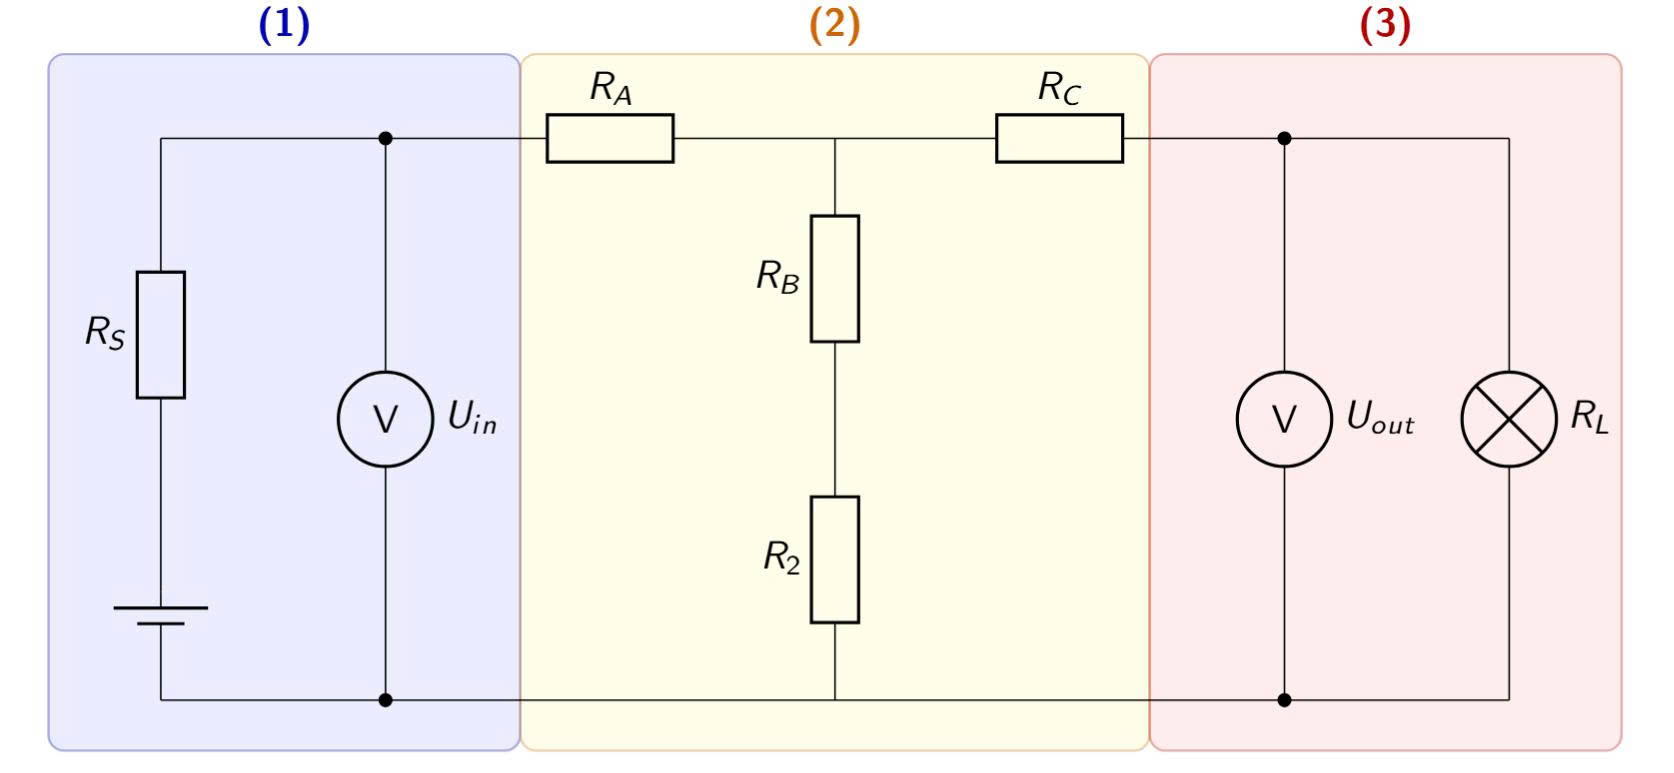
\includegraphics[width=0.8\textwidth]{Problem_3/Image/P3_I3.png}
\caption{Mạch chuyển đổi sao - tam giác}
\end{figure}

\begin{equation}
R_A=\frac{R_1R_4}{R_1+R_3+R_4}
\end{equation}

\begin{equation}
R_B=\frac{R_1R_3}{R_1+R_3+R_4}
\end{equation}

\begin{equation}
R_C=\frac{R_3R_4}{R_1+R_3+R_4}
\end{equation}


Thế lần lượt các phương trình điện trở đã tìm được ở mạch T:

\begin{equation}
\label{eq:d1}
R_A=\frac{K-1}{K+1}=\frac{R_1R_4}{R_1+R_3+R_4} R_L
\end{equation}

\begin{equation}
\label{eq:d2}
R_C=\frac{K-1}{K+1}=\frac{R_1R_4}{R_1+R_3+R_4} R_L
\end{equation}

\begin{equation}
\frac{2K}{K^2-1} R_L=R_B+R_2=\frac{R_1R_3}{R_1+R_3+R_4}+R_2
\end{equation}

Với hai phương trình \eqref{eq:d1} và \eqref{eq:d2} ta có:

\begin{equation}
\Rightarrow R_1=R_3
\end{equation}

Đặt $R_4=fR_1$:

\begin{equation}
\Rightarrow \frac{K-1}{K+1} R_L=\frac{R_1R_4}{R_1+R_3+R_4}
\end{equation}

\begin{equation}
\Rightarrow \frac{K-1}{2+K-1} R_L=\frac{fR_1}{2+f}
\end{equation}

Với $R_1$ = $R_3$ = $R_L$, ta có $f=K-1$. Từ đó ta tìm được $R_4$:

\begin{equation}
\Rightarrow R_4=(K-1)R_L
\end{equation}

Ta tìm $R_2$:

\begin{equation}
\begin{aligned}
R_2 &= \frac{2K}{K^2-1} R_L-\frac{R_1R_3}{R_1+R_3+R_4}
\\ &= \frac{2K}{K^2-1} R_L-\frac{1}{K+1} R_L
\\ &= \frac{R_L}{K-1}
\end{aligned}
\end{equation}

Thế giá trị $K$ và $R_L$ vào; với $K=\left(\frac{1}{10\%}\right)^{1/2}=\sqrt{10}$ và $R_L=50\ \mathrm{ohm}$:

\begin{equation*}
\Rightarrow \left\{
\begin{aligned}
R_2&=\frac{R_L} {K-1} \approx 23.12\,\Omega,\\
R_4&=(K-1) R_L \approx 108.11\,\Omega
\end{aligned}
\right. 
\end{equation*}

Ta nhận thấy rằng ở mạch suy hao T tồn tại ba điện trở cần tùy chỉnh liên tiếp để đạt được độ suy hao mong muốn. Tuy nhiên, để đảm bảo tối ưu hóa đường truyền thì ở bridged-T chỉ còn hai điện trở $R_2$ và $R_4$ cần thay đổi độ suy hao. Đồng thời, khi thay đổi giá trị suy hao thì điều kiện \textbf{$R_2R_4 = R_L^2 = {const}$}, nghĩa là đáp ứng được một mối quan hệ như đề bài yêu cầu mà không phụ thuộc vào giá trị tỷ lệ công suất.

\emph{Lời bình:} 
Câu a của bài tập này được phỏng theo một tính chất rất thú vị rằng: khi ta đặt một nguồn áp(dòng điện đi vào) vào một trong hai đầu của mạch điện bất kỳ thì áp tải(dòng điện đi ra) luôn đưa ra một giá trị nhất định. Điều này là do cả hai luôn tỷ lệ với nhau thông qua điện dẫn tương hỗ, khi thay đổi vị trí của nguồn áp thì hệ số này vẫn không đổi(Bạn có thể tìm hiểu sâu thêm về mạng hai cửa tuyến tính để hiểu rõ hơn về tính chất này).

Ngoài cấu trúc suy hao được giới thiệu trong bài tập này, ta còn có các dạng cấu trúc phổ biến khác như Pi-pad hoặc L-pad(Cấu trúc của bài 1 là T-pad), đặc biệt là cấu trúc mạch Pi có thể được biến đổi từ mạch T thông qua phép tương đương sao - tam giác cơ bản. Ý nghĩa lớn nhất của các cấu trúc này(như đã đề cập ở trên) là để giúp hấp thụ bớt năng lượng tín hiệu đi qua và tín hiệu phản xạ trở lại. Điều này giúp cô lập các tầng khuếch đại, ngăn không cho tầng sau tác động ngược trở lại tầng trước. Trong bài này cũng đã sử dụng tỷ lệ giữa công suất điện trở thiết bị so với nguồn thay cho một thuật ngữ phổ biến hơn được gọi là \emph{độ suy hao}. Công thức của độ suy hao được tính như sau: 
\begin{equation}
    dB_v = 20log(\frac{V_{out}}{V_{in}})
\end{equation}
Trong đó: $V_{in}$ và $V_{out}$ lần lượt là nguồn áp vào - ra, $dB_v$ là độ suy hao của cấu trúc.
\vspace{0.5cm}

\noindent \textbf{\large Phổ điểm}
\begin{center}
\renewcommand{\arraystretch}{1.5}
\begin{tabularx}{\textwidth}{|c|X|c|}
\hline
\textbf{Phần} & \textbf{Nội dung} & \textbf{Điểm thành phần} \\ \hline
a & Thiết lập đúng mối liên hệ giữa điện trở $R_S$ và $R_{\mathrm{td}}$. & 0.25 \\ \cline{2-3} 
 & Chứng minh được giá trị $U_{out}$ luôn không đổi. & 0.75 \\ \hline
b & Nêu được sự phụ thuộc của các điện trở vào độ suy hao & 0.5 \\ \cline{2-3} 
 & Tính toán đúng kết quả của từng giá trị điện trở & 0.25 \\ \hline
c & Thiết lập được phương trình tổng quát của các điện trở & 0.5 \\ \cline{2-3} 
 & Chứng minh không có ba điện trở nào đáp ứng được yêu cầu & 0.5 \\ \cline{2-3}  \hline
d & Thiết lập được phương trình tổng quát của các điện trở thông qua mạch tương đương sao - tam giác (hoặc cách khác) & 0.5 \\ \cline{2-3} 
 & Tính toán đúng kết quả của từng giá trị điện trở & 0.25 \\ \hline
e & Nêu được cách sử dụng biến trở đôi ở mạch Bridged-T cho hai điện trở $R_2$ và $R_4$ & 0.5 \\ \cline{2-3} 

\multicolumn{2}{|r|}{\textbf{Tổng điểm}} & \textbf{4.0} \\ \hline
\end{tabularx}
\end{center}